\documentclass[a4aper,pagesize]{article}
\usepackage[utf8]{inputenc}
\usepackage[T1]{fontenc}
\usepackage[english]{babel}
\usepackage{enumitem}
\usepackage{amsmath}
\usepackage{amssymb}
\usepackage{amsthm}
\usepackage{breqn}
\usepackage{graphicx}
\usepackage{pdfpages}
\usepackage{float}
\usepackage{subfigure}
\usepackage{subfigure}
\usepackage{stmaryrd}
\usepackage{tikz}
\usetikzlibrary{decorations.pathreplacing}
\usepackage{wrapfig}
\usepackage{blindtext}

\theoremstyle{definition}
\newtheorem{mydef}{Definition}[section]
\theoremstyle{plain}
\newtheorem{thm}[mydef]{Theorem}
\theoremstyle{remark}
\newtheorem{bem}{Bemerkung}[section]

\newcommand{\func}[3]{$ #1 : #2 \rightarrow #3 $}
\newcommand{\xvecn}[1]{$( #1 _1,...,#1 _n)$}
\newcommand{\xser}[2]{$ #1 _1,...,#1 _#2$}
\newcommand{\ser}[2]{ #1 _1,...,#1 _#2}
\newcommand{\xvec}[2][n]{$( #2 _1,...,#2 _{#1})$}
\newcommand{\RR}{\mathbb{R}}
\newcommand{\NN}{\mathbb{N}}
\newcommand{\PP}{\mathbb{P}}
\newcommand{\EE}{\mathbb{E}}
\newcommand{\cO}{\mathcal{O}}
\newcommand{\cA}{\mathcal{A}}
\newcommand{\cB}{\mathcal{B}}
\newcommand{\cF}{\mathcal{F}}
\newcommand{\Borel}{\mathcal{B}}
\newcommand{\bernulli}{\mathrm{Ber}}
\newcommand{\uniform}{\mathrm{U}}
\newcommand{\indicator}{\mathbbm{1}}
\newcommand{\pderiv}[2]{\frac{\partial #1}{\partial #2}}
\newcommand{\di}{\mathrm{d}}
\renewcommand{\hat}{\widehat}

%setzt den hervorhebungsstil
\DeclareTextFontCommand{\emph}{\bfseries}

%verhindert einrückung bei neuem absatz
%\setlength{\parindent}{0em} 

\title{On the ADI Method}
\date{\today}
\author{Thomas Steindl, Daylen Thimm}

\begin{document}

\maketitle

\section*{Introducion}
This work discusses possible numerical schemes to solve the two dimensional heat equation with homogeneous Dirichlet boundary conditions. This means we are looking for a function
\begin{align}
	T: \Omega \times [0,\infty) &\rightarrow \RR\\
	(x,t)  &\mapsto T(x,t)
\end{align} that fulfills
\begin{align}
	\partial_t T(x,t) &= \partial_{x^2} T(x,t) + \partial_{y^2} T(x,t) &\text{for } x\in\Omega, t\in[0,\infty)\\
	T(x,t) &= 0 &\text{for } x\in\partial \Omega, t\in[0,\infty)\\
	T(x, 0) &= T_0 &\text{for } x\in\Omega, t\in[0,\infty),
\end{align}
where $\Omega = [-1,1]^2$.\\

Three methods are compared: the explicit scheme, the implicit scheme and the alternating direction implicit (ADI) scheme. The calculations in the following show that the explicit suffers from a very limiting CFL condition. The full implicit scheme overcomes this condition and is shown to be unconditionally stable. Nevertheless the full implicit scheme has the disadvantage in solving a relatively computation intensive system of linear equations. The ADI scheme unites the best qualities of both the before mentioned. It is unconditionally stable and the system of linear equations has tridiagonal form and can therefor be solved using Thomas algorithm which is very efficient.

\section{Explicit Scheme}
The explicit scheme for the two dimensional heat equation is
\begin{align}
	&\frac{T_{j,k}^{n+1} - T_{j,k}^{n}}{\Delta t}
	= \frac{T_{j-1,k}^{n} - 2 T_{j,k}^{n} + T_{j+1,k}^{n}}{(\Delta x)^2}
	+ \frac{T_{j,k-1}^{n} - 2 T_{j,k}^{n} + T_{j,k+1}^{n}}{(\Delta y)^2}
\Leftrightarrow\\
\Leftrightarrow
	&T_{j,k}^{n+1}
	= T_{j,k}^{n}
	+ \frac{1}{\rho} \left(
		T_{j-1,k}^{n}
		+ T_{j+1,k}^{n}
		+ T_{j,k-1}^{n}
		+ T_{j,k+1}^{n}
		- 4 T_{j,k}^{n}
	\right).
\end{align}
The value of $T_{j,k}^{n+1}$ can directly be calculated.
\subsection{Van Neumann Stability Analysis: Explicit Scheme}
Let us assume $\Delta x = \Delta y =: h$ and set $\rho = \frac{h^2}{\Delta t}$. We begin our van Neumann stability analysis by inserting the Fourier series
\begin{equation}
	T_{j,k}^n = \sum_{p,q = 0}^{N-1} \hat{T}^n_{p,q} e^{ipx_j + iqy_k}
\end{equation}
into the numerical scheme. We obtain
\begin{equation}
	\begin{split}
		\sum_{p,q = 0}^{N-1} \hat{T}^{n+1}_{p,q} e^{i(px_{j} + qy_{k})} =
		\sum_{p,q = 0}^{N-1} (
			&\hat{T}^{n}_{p,q} e^{i(px_{j} + qy_{k})} +
			\frac{1}{\rho} (
			  	  \hat{T}^{n}_{p,q} e^{i(px_{j-1} qy_{k})}
				+ \hat{T}^{n}_{p,q} e^{i(px_{j+1} + qy_{k})} + \\
			   &+ \hat{T}^{n}_{p,q} e^{i(px_{j} + qy_{k-1})}
				+ \hat{T}^{n}_{p,q} e^{i(px_{j} + qy_{k+1})}
				-  4 \hat{T}^{n}_{p,q} e^{i(px_{j} + qy_{k})}
			)
		).
	\end{split}
\end{equation}
Using that $x_{j+1} = {x_j} + h$ and $x_{j-1} = {x_j} - h$ and that the discretization in $x$ and $y$ are the same we get
\begin{equation}
	\sum_{p,q = 0}^{N-1}(
		  \hat{T}^{n+1}_{p,q}
		- \hat{T}^{n}_{p,q}
		-\frac{1}{\rho} (
			  \hat{T}^{n}_{p,q} e^{-iph}
			+ \hat{T}^{n}_{p,q} e^{iph}
		    + \hat{T}^{n}_{p,q} e^{-iqh}
			+ \hat{T}^{n}_{p,q} e^{iqh}
			-  4 \hat{T}^{n}_{p,q}
		)
	)\, e^{i(px_{j} + qy_{k})} = 0
\end{equation}
and because $(e^{i(px_{j} + qy_{k})})_{j,k \in \{0, ..., N-1\}}$ is a basis of the trigonometrical polynomials of degree $N$ in two variables we have for all $p,q \in \{0, \dots, N-1\}$ that
\begin{align*}
	  &\hat{T}^{n+1}_{p,q}
	- \hat{T}^{n}_{p,q}
	-\frac{1}{\rho} \left(
		  \hat{T}^{n}_{p,q} e^{-iph}
		+ \hat{T}^{n}_{p,q} e^{iph}
	    + \hat{T}^{n}_{p,q} e^{-iqh}
		+ \hat{T}^{n}_{p,q} e^{iqh}
		-  4 \hat{T}^{n}_{p,q}
	\right)= 0
&\Leftrightarrow\\
\Leftrightarrow
	  &\hat{T}^{n+1}_{p,q} =
      \hat{T}^{n}_{p,q}
	 +\frac{1}{\rho} \left(
		  \hat{T}^{n}_{p,q} e^{-iph}
		+ \hat{T}^{n}_{p,q} e^{iph}
	    + \hat{T}^{n}_{p,q} e^{-iqh}
		+ \hat{T}^{n}_{p,q} e^{iqh}
		-  4 \hat{T}^{n}_{p,q}
	\right)
&\Leftrightarrow\\
\Leftrightarrow
	  &\hat{T}^{n+1}_{p,q} =
      \hat{T}^{n}_{p,q}\left(
      1
	 +\frac{1}{\rho} \left(
		  e^{-iph}
		+ e^{iph}
	    + e^{-qh}
		+ e^{qh}
		-  4
	    \right)
	\right)
&\Leftrightarrow\\
\Leftrightarrow
	  &\hat{T}^{n+1}_{p,q} =
      \hat{T}^{n}_{p,q}\left(
      1
	 +\frac{1}{\rho} \left(
		  2\cos(ph)
	    + 2\cos(qh)
	    - 4
	    \right)
	\right)
&\Leftrightarrow\\
\Leftrightarrow
	  &\hat{T}^{n+1}_{p,q} =
      \hat{T}^{n}_{p,q}\underbrace{\left(
      1
	 -\frac{4}{\rho} \left(
	      \sin^2\left(\frac{ph}{2}\right)
	    + \sin^2\left(\frac{qh}{2}\right)
	    \right)
	  \right)}_{=:G_{p,q}},
\end{align*}
where in the last step the identity $\sin^2(\alpha/2) = \frac{1}{2}(1-\cos(\alpha))$ was used. For van Neumann stability we need that $|G_{p,q}|<1$. We therefor want to find conditions on $\Delta t$ and $h$ such that
\begin{equation}
-1 \le
	1-\frac{4}{\rho} \left(
		  \sin^2\left(\frac{ph}{2}\right)
	    + \sin^2\left(\frac{qh}{2}\right)
	\right)
	\le 1.
\end{equation}
The right hand side inequality is trivial and for the left hand side inequality we need that $\rho \geq 4$. This gives us the CFL condition
\begin{equation}
	\frac{h^2}{\Delta t} = \rho \geq 4 \Leftrightarrow \Delta t \leq \frac{h^2}{4} = \frac{1}{4N^2}.
\end{equation}
We conclude that $4N^2t$ time steps are needed to integrate up to a time $t$. Since for every of the $N^2$ many grid points $7$ arithmetic calculations are needed this totals to $28N^4t$ operations are needed. This demonstrates the problem with using an explicit method. We would like to be able to make larger time steps. Implicit schemes can help with this.

\section{Implicit Scheme}
The implicit scheme for the two dimensional heat equation is
\begin{align}
	&\frac{T_{j,k}^{n+1} - T_{j,k}^{n}}{\Delta t}
	= \frac{T_{j-1,k}^{n+1} - 2 T_{j,k}^{n+1} + T_{j+1,k}^{n+1}}{(\Delta x)^2}
	+ \frac{T_{j,k-1}^{n+1} - 2 T_{j,k}^{n+1} + T_{j,k+1}^{n+1}}{(\Delta y)^2}
\Leftrightarrow\\
\Leftrightarrow
	&T_{j,k}^{n+1}
	= T_{j,k}^{n}
	+ \frac{1}{\rho} \left(
		T_{j-1,k}^{n+1}
		+ T_{j+1,k}^{n+1}
		+ T_{j,k-1}^{n+1}
		+ T_{j,k+1}^{n+1}
		- 4 T_{j,k}^{n+1}
	\right).
\end{align}

\subsection{Van Neumann Stability Analysis: Implicit Scheme}
Assuming $\Delta x = \Delta y =: h$ and setting $\rho = \frac{h^2}{\Delta t}$. Again, we begin our Van Neumann stability analysis by inserting the Fourier series
\begin{equation}
	T_{j,k}^n = \sum_{p,q = 0}^{N-1} \hat{T}^n_{p,q} e^{ipx_j + iqy_k}
\end{equation}
into the numerical stencil. We bring all terms to one side of the equation and again by using $x_{j+1} = {x_j} + h$ and $x_{j-1} = {x_j} - h$ and that the discretization in $x$ and $y$ are the same and also by placing the exponential outside of the brackets we get
\begin{dmath}
	\sum_{p,q = 0}^{N-1} \left(
		\hat{T}_{p,q}^{n+1}
		-\hat{T}_{p,q}^{n}
		-\frac{1}{\rho}\left(
			\hat{T}_{p,q}^{n+1} e^{-iph}
			+ \hat{T}_{p,q}^{n+1} e^{iph}
			+ \hat{T}_{p,q}^{n+1} e^{-iqh}+\\
			+ \hat{T}_{p,q}^{n+1} e^{iph}
			- 4\hat{T}_{p,q}^{n+1}
		\right)
	\right)
	e^{i(px_j + qy_k)}
	=
	0.
\end{dmath}
Again because the occurring exponentials is a basis of the trigonometrical polynomials the exponentials coefficients must be zero. From this we calculate
\begin{dmath}
	\hat{T}_{p,q}^{n}
	=
	\hat{T}_{p,q}^{n+1}
	-\frac{1}{\rho}\left(
		\hat{T}_{p,q}^{n+1} e^{-iph}
		+ \hat{T}_{p,q}^{n+1} e^{iph}
		+ \hat{T}_{p,q}^{n+1} e^{-iqh}
		+ \hat{T}_{p,q}^{n+1} e^{iph}
		- 4\hat{T}_{p,q}^{n+1}
	\right)
	=
	\hat{T}_{p,q}^{n+1}\left(
		1
		-\frac{1}{\rho}\left(
			e^{-iph}
			+e^{iph}
			+e^{-iqh}
			+e^{iph}
			- 4
		\right)
	\right)
	=
	\hat{T}_{p,q}^{n+1}\left(
		1
		-\frac{1}{\rho}\left(
			2\cos(ph)
			+ 2\cos(qh)
			- 4
		\right)
	\right)
	=
	\hat{T}_{p,q}^{n+1}\left(
		1
		-\frac{4}{\rho}\left(
			\sin^2\left(\frac{ph}{2}\right)
			+ \sin^2\left(\frac{qh}{2}\right)
		\right)
	\right),
\end{dmath}
which is equivalent to
\begin{dmath}
	\hat{T}_{p,q}^{n+1}
	=
	\hat{T}_{p,q}^{n}
	\underbrace{
		\frac{1}{
			1
			-\frac{4}{\rho}\left(
				\sin^2\left(\frac{ph}{2}\right)
				+ \sin^2\left(\frac{qh}{2}\right)
			\right)
		}.
	}_{=:G_{p,q}}
\end{dmath}
Clearly here $|G_{p,q}|\leq1$ is always fulfilled. Therefore the implicit scheme is unconditionally stable and hence no CFL condition is existent. Solving the equations is usually done with some iterative method like successive overrelaxation methods. It can be shown that for every time step the amount of numerical computations is proportional to $N^2$.

\section{ADI Scheme}
The alternating direction implicit (ADI) method consists of the two half steps
\begin{align}
	\frac{T_{j,k}^{2n+1} - T_{j,k}^{2n}}{\Delta t}
	&= \frac{T_{j-1,k}^{2n+1} - 2 T_{j,k}^{2n+1} + T_{j+1,k}^{2n+1}}{(\Delta x)^2}
	+ \frac{T_{j,k-1}^{2n} - 2 T_{j,k}^{2n} + T_{j,k+1}^{2n}}{(\Delta y)^2}
\\
	\frac{T_{j,k}^{2n+2} - T_{j,k}^{2n+1}}{\Delta t}
	&= \frac{T_{j-1,k}^{2n+1} - 2 T_{j,k}^{2n+1} + T_{j+1,k}^{2n+1}}{(\Delta x)^2}
	+ \frac{T_{j-1,k}^{2n+2} - 2 T_{j,k}^{2n+2} + T_{j+1,k}^{2n+2}}{(\Delta y)^2}.
\end{align}
The idea here is to have an explicit scheme in one component and an implicit in the other for each half step. Where the implicit scheme is used alternates with each half step.

\subsection{Van Neumann Stability Analysis: ADI Scheme}
Due to the fact that these schemes are identical except for an index shift and a transposition of the $x$ and $y$ direction we only consider the first half step for the stability analysis, the second one can then easily be deduced. Using the same strategy as in the previous examples we begin by bringing all terms to one side and separating the terms of the $2n$-th step from the ones of the $(2n+1)$-th step. This leaves us with
\begin{equation}
	T_{j,k}^{2n+1}
	- \frac{1}{\rho}\left(
		T_{j-1,k}^{2n+1}
		-2T_{j,k}^{2n+1}
		+T_{j+1,k}^{2n+1}
	\right)
	-T_{j,k}^{2n}
	- \frac{1}{\rho}\left(
		T_{j-1,k}^{2n}
		-2T_{j,k}^{2n}
		+T_{j,k+1}^{2n}
	\right)
	=
	0,
\end{equation}
assuming $\Delta x = \Delta y =: h$ and setting $\rho = \frac{h^2}{\Delta t}$. Again we start by inserting the Fourier series
\begin{equation}
	T_{j,k}^n = \sum_{p,q = 0}^{N-1} \hat{T}^n_{p,q} e^{ipx_j + iqy_k}
\end{equation}
into the numerical stencil. We bring all terms to one side of the equation and again by using $x_{j+1} = {x_j} + h$ and $x_{j-1} = {x_j} - h$ and that the discretization in $x$ and $y$ are the same and also by placing the exponential outside of the brackets we get
\begin{dmath}
	\sum_{p,q = 0}^{N-1}\left(
		\hat{T}_{p,q}^{2n+1}
		-\frac{1}{\rho}\left(
			\hat{T}_{p,q}^{2n+1} e^{-iph}
			- 2 \hat{T}_{p,q}^{2n+1}
			+ \hat{T}_{p,q}^{2n+1} e^{iph}
		\right)
		-\\
		-\hat{T}_{p,q}^{2n+1}
		-\frac{1}{\rho}\left(
			\hat{T}_{p,q}^{2n} e^{-iph}
			- 2 \hat{T}_{p,q}^{2n}
			+ \hat{T}_{p,q}^{2n} e^{iph}
		\right)
	\right)
	e^{i(px_j + qy_k)}
	=
	0.
\end{dmath}
Because $(e^{i(px_{j} + qy_{k})})_{j,k \in \{0, ..., N-1\}}$ is a basis of the trigonometrical polynomials of degree $N$ in two variables we have for all $p,q \in \{0, \dots, N-1\}$ that the coefficients of the exponentials must be zero. Rearranging the terms gives us that for all $p,q \in \{0, \dots, N-1\}$ that
\begin{align}
	&\hat{T}_{p,q}^{2n+1}
	\left(
		1
		-\frac{1}{\rho}\left(
			e^{-iph}
			+ e^{iph}
			- 2
		\right)
	\right)
	=
	\hat{T}_{p,q}^{2n}
	\left(
		1
		+\frac{1}{\rho}\left(
			e^{-iqh}
			+ e^{iqh}
			- 2
		\right)
	\right)
\Leftrightarrow\\
\Leftrightarrow&
	\hat{T}_{p,q}^{2n+1}
	=
	\hat{T}_{p,q}^{2n}
	\frac{
		1
		-\frac{1}{\rho}\left(
			e^{-iqh}
			+ e^{iqh}
			- 2
		\right)
	}{
		1
		+\frac{1}{\rho}\left(
			e^{-iph}
			+ e^{iph}
			- 2
		\right)
	}
	=
	\hat{T}_{p,q}^{2n+1}
	=
	\hat{T}_{p,q}^{2n}
	\frac{
		1-\frac{1}{\rho}(2\cos(ph)- 2)
	}{
		1-\frac{1}{\rho}(2\cos(qh)- 2)
	}
\Leftrightarrow\\
\Leftrightarrow&
	\hat{T}_{p,q}^{2n+1}
	=
	\hat{T}_{p,q}^{2n}
	\frac{
		1-\frac{4}{\rho}\left(\sin^2\left(\frac{ph}{2}\right)\right)
	}{
		1+\frac{4}{\rho}\left(\sin^2\left(\frac{qh}{2}\right)\right)
	},
\end{align}
where we usewhere we used $\sin^2(\alpha/2) = \frac{1}{2}(1-\cos(\alpha))$ in the last step. expanding the fraction by $\rho$ finally leaves us with
\begin{equation}
	\hat{T}_{p,q}^{2n+1}
	=
	\hat{T}_{p,q}^{2n}
	\underbrace{
		\frac{
			\rho-4\sin^2\left(\frac{ph}{2}\right)
		}{
			\rho+4\sin^2\left(\frac{qh}{2}\right)
		}
	}_{=:G_{p,q}^{(1)}}.
	\label{eq:AdiNeumann1}
\end{equation}
By performing an index shift and switching the two space dimensions i.e.
\begin{eqnarray*}
	2n &\rightarrow &2n+1\\
	2n+1 &\rightarrow &2n+2\\
	p &\rightarrow &q\\
	q &\rightarrow &p
\end{eqnarray*}
we get the analogue equation for the second half step of the ADI method.
\begin{equation}
	\hat{T}_{p,q}^{2n+2}
	=
	\hat{T}_{p,q}^{2n+1}
	\underbrace{
		\frac{
			\rho-4\sin^2\left(\frac{qh}{2}\right)
		}{
			\rho+4\sin^2\left(\frac{ph}{2}\right)
		}
	}_{=:G_{p,q}^{(2)}}.
\end{equation}
Unfortunately separately these steps are highly unstable as there exist values for $p,q$ and $\rho$ such that $|G_{p,q}|>1$, for example for $\rho = 1$, $q = 1$, $p = 0$ and $h = \pi$ we have $G_{p,q}^{(1)} = -3$. Also no constraint is obvious to bound $G_{p,q}^{(1)}$ by unity. In the contrary, when using both half steps alternately we get
\begin{equation}
	\hat{T}_{p,q}^{2n+2}
	=
	\hat{T}_{p,q}^{2n}
	\underbrace{
		\left(
			\frac{
				\rho-4\sin^2\left(\frac{qh}{2}\right)
			}{
				\rho+4\sin^2\left(\frac{ph}{2}\right)
			}
			\cdot
			\frac{
				\rho-4\sin^2\left(\frac{ph}{2}\right)
			}{
				\rho+4\sin^2\left(\frac{qh}{2}\right)
			}
		\right)
	}_{=:G_{p,q}},
\end{equation}
where $G_{p,q}$ is bounded by unity (compare the nominator and denominator of different fractions respectively) and hence the ADI method is stable.

\subsection{Solving the Linear System}
For the ADI scheme we need to solve $N$ sets of $N$ simultaneous equations of the form

\begin{equation}
	T_{i-1,j}^{2n+1} - (2+\rho)T_{i,j} + T_{i+1,j}^{2n+1} = -T_{i,j-1}^{2n} + (2-\rho)T_{i,j}^{2n} - T_{i,j+1}^{2n}.
\end{equation}
This can be written as a matrix vector multiplication by flattening the 2D discretization. We get a system of the tridiagonal form
\begin{equation}
\scalebox{0.8}{
	\begin{bmatrix}
			\ddots & \ddots & 0 & 0 & 0 \\
			\ddots & -(2+\rho) & 1 & 0 & 0 \\
			0 & 1 &-(2+\rho) & 1 & 0\\
			0 & 0 & 1 &-(2+\rho) & \ddots\\
			0 & 0 & 0 & \ddots & \ddots
	\end{bmatrix}
	\begin{bmatrix}
		\vdots\\
		T_{i-1,j}^{2n+1}\\
		T_{i,j}^{2n+1}\\
		T_{i+1,j}^{2n+1}\\
		\vdots
	\end{bmatrix}
	=
	\begin{bmatrix}
		\vdots\\
		-T_{i-1,j-1}^{2n} + (2-\rho)T_{i-1,j}^{2n}-T_{i-1,j+1}^{2n}\\
		-T_{i,j-1}^{2n} + (2-\rho)T_{i,j}^{2n}-T_{i,j+1}^{2n}\\
		-T_{i+1,j-1}^{2n} + (2-\rho)T_{i+1,j}^{2n}-T_{i+1,j+1}^{2n}\\
		\vdots
	\end{bmatrix}
}
\end{equation}
which can be efficiently solved using Thomas algorithm.

\section{Analytic Solution}
In the case of the simple heat equation it is possible to derive an analytic solution. This is useful for verifying the numerically calculated approximations to it and checking the numerical error.\\

We consider the heat equation
\begin{align}
    \frac{\partial^2 T}{ \partial x ^2} + \frac{\partial^2 T}{ \partial y ^2} = \frac{\partial T}{ \partial t}
\end{align}
in the range $0 \leq x \leq 1$ and  $0 \leq y \leq 1$ with the boundary conditions
\begin{align}
    T(0,y,t) = T(1, y, t) = T(x, 0, t) = T(x, 1, t) = 0
\end{align}
and the initial state $T =1$. We solve the equation be seperating the variables, such that
\begin{align}
    T(x, y, t) = v(x, y) * \Tilde{T}(t) \\
    \Longrightarrow \Tilde{T}\left(\frac{\partial^2 v}{ \partial x ^2} + \frac{\partial^2 v}{ \partial y ^2}  \right) = v \frac{\partial \Tilde{T}}{ \partial t}.
\end{align}
Thus,
\begin{align}
\frac{v_{xx} + v_{yy}}{v} = \frac{\Tilde{T}'}{\Tilde{T}} \overset{!}{=} -\lambda \quad \quad {\rm constant},
\end{align}
where, e.g.  $v_{xx} = \frac{\partial^2 T}{ \partial x ^2}$ and e.g. $\Tilde{T}' = \frac{\partial \Tilde{T}(t)}{\partial t}$.

This is a Sturm-Luisville problem for $v(x, y)$ with the equation
\begin{align}
    v_{xx} + v_{yy} + \lambda v = 0
\end{align}
with the boundary conditions
\begin{align}
    v(0,y,t) = v(1, y, t) = v(x, 0, t) = v(x, 1, t) = 0.
\end{align}
Seperating the variables according to
\begin{align}
    v(x, y) = X(x) Y(y)
\end{align}
yields
\begin{align}
    X''Y + XY''+ XY\lambda = 0\\
    \Longrightarrow  X''Y + XY''=- XY\lambda .
\end{align}
Hence, we have that
\begin{align}
    \frac{X''}{X} + \frac{Y''}{Y} = -\lambda \\
    \longrightarrow \frac{Y''}{Y} + \lambda. = -\frac{X''}{X} \overset{!}{=} \mu \quad \quad{\rm constant}.
\end{align}
For $X(x)$ this results in the equation
\begin{align}
    X'' + \mu X = 0
\end{align}
with boundary conditions
\begin{align}
    X(0) = X(1) = 0.
\end{align}
The solution for the differential equation is
\begin{align}
    X(x) = A \cos(\sqrt{\mu}x) + B\sin(\sqrt{\mu}x).
\end{align}
Inserting the boundary conditions yields
\begin{align}
    &X(0) = 0 = A \\
    X(1) = 0 = A &\cos(\sqrt{\mu}) + B\sin(\sqrt{\mu}) = B\sin(\sqrt{\mu}).
\end{align}
Since we are looking for a non-trivial solution, $B \neq 0$, we have that
\begin{align}
    &\sin(\sqrt{\mu}) \overset{!}{=} 0 \\
    \Longrightarrow X_n(x) = B_n \sin(n\pi  x) \quad& {\rm for} \quad \mu_n = n^2\pi^2 \quad \forall \,n = 1, 2, 3, ...
\end{align}
For $Y(y)$ we have the equation
\begin{align}
    X'' + \nu X = 0 \quad \quad {\rm with} \quad \nu = \lambda - \mu
\end{align}
and the boundary conditions
\begin{align}
    Y(0) = Y(1) = 0.
\end{align}
The solution to the differential equation is again
\begin{align}
    Y(y) = \Tilde{A} \cos(\sqrt{\nu}y) + \Tilde{B}\sin(\sqrt{\nu}y).
\end{align}
Inserting the boundary conditions yields
\begin{align}
    &Y(0) = 0 = \Tilde{A} \\
    Y(1) = 0 = \Tilde{A} &\cos(\sqrt{\mu}) + \Tilde{B}\sin(\sqrt{\mu}) = \Tilde{B}\sin(\sqrt{\mu}).
\end{align}
Since we are again looking for a non-trivial solution we have
\begin{align}
    &\sin(\sqrt{\nu}) \overset{!}{=} 0 \\
    \Longrightarrow Y_m(y) = \Tilde{B}_m \sin(m\pi  y)& \quad {\rm for} \quad \mu_m = m^2\pi^2 \quad \forall \,m = 1, 2, 3, ...
\end{align}
The solution for $v(x,y)$ is hence
\begin{align}
    v(x,y) = X(x)Y(y) = A_{nm} \sin(n\pi  x) \sin(m\pi  y),
\end{align}
where $A_{nm} = B_n \Tilde{B}_m$.

For $\Tilde{T}$ it follows that
\begin{align}
    &\frac{\Tilde{T}'}{\Tilde{T}} = -\lambda \quad \quad {\rm with} \quad \lambda = \nu_m + \mu_n \\
    &\Longrightarrow \Tilde{T}' = -\lambda \Tilde{T}
\end{align}
Hence, the solution is
\begin{align}
    T(t) &= \exp(-\lambda t) \\
    &=\exp(-(\nu_m + \mu_n)t) \\
    &= \exp(-(m^2+ n^2)\pi^2t) \quad \forall \,m,n = 1, 2, 3, ...
\end{align}

For $T(x, y, t)$ we have
\begin{align}
    T(x, y, t) &= \sum_{m=1}^\infty\sum_{n=1}^\infty T_{m n}(x, y, t) \\
    &= \sum_{m=1}^\infty\sum_{n=1}^\infty A_{m n}\sin(n\pi  x) \sin(m\pi  y)\exp(-(m^2+ n^2)\pi^2t)
\end{align}
The initial conditions are
\begin{align}
    1 = \sum_{m=1}^\infty\sum_{n=1}^\infty A_{m n}\sin(n\pi  x) \sin(m\pi  y)\
\end{align}
from which we can find $A_{mn}$ using the orthogonality relations for $\sin$. We have that
\begin{align}
    A_{mn} &= 4 \int_0^1 \int_0^1\sin(n\pi  x) \sin(m\pi  y)\mathrm{d}x\mathrm{d}y \\
    &= 4 \int_0^1 \sin(n\pi  x)\mathrm{d}x\int_0^1 \sin(m\pi  y)\mathrm{d}y \\
    &= 4 \frac{1}{n \pi} \cos(n\pi) \frac{1}{m \pi} \cos(m\pi) \\
    &=\frac{4}{nm\pi^2}\left((-1)^n -1\right)\left((-1)^ -1\right).
\end{align}
Which reduces to
\begin{align}
    A_{2m2n} &=0 \\
    A_{(2m-1)(2n-1)} = \frac{16}{(2m-1)(2n-1)\pi^2}.
\end{align}
Hence, the solution for the heat equation with our boundary condition and initial conditions is
\begin{align}
    T(x, y, t) = \sum_{m=1}^\infty\sum_{n=1}^\infty \frac{16}{(2m-1)(2n-1)\pi^2} \sin(n\pi  x) \sin(m\pi  y)\exp(-(m^2+ n^2)\pi^2t)
\end{align}



\section{Implementation}
All the three methods were implemented in python. In the following diagram the computation time and the corresponding errors calculated using the analytic solution are shown. One can see that the ADI method severely outperforms the other two methods.


\begin{figure}[h!]
\centering
	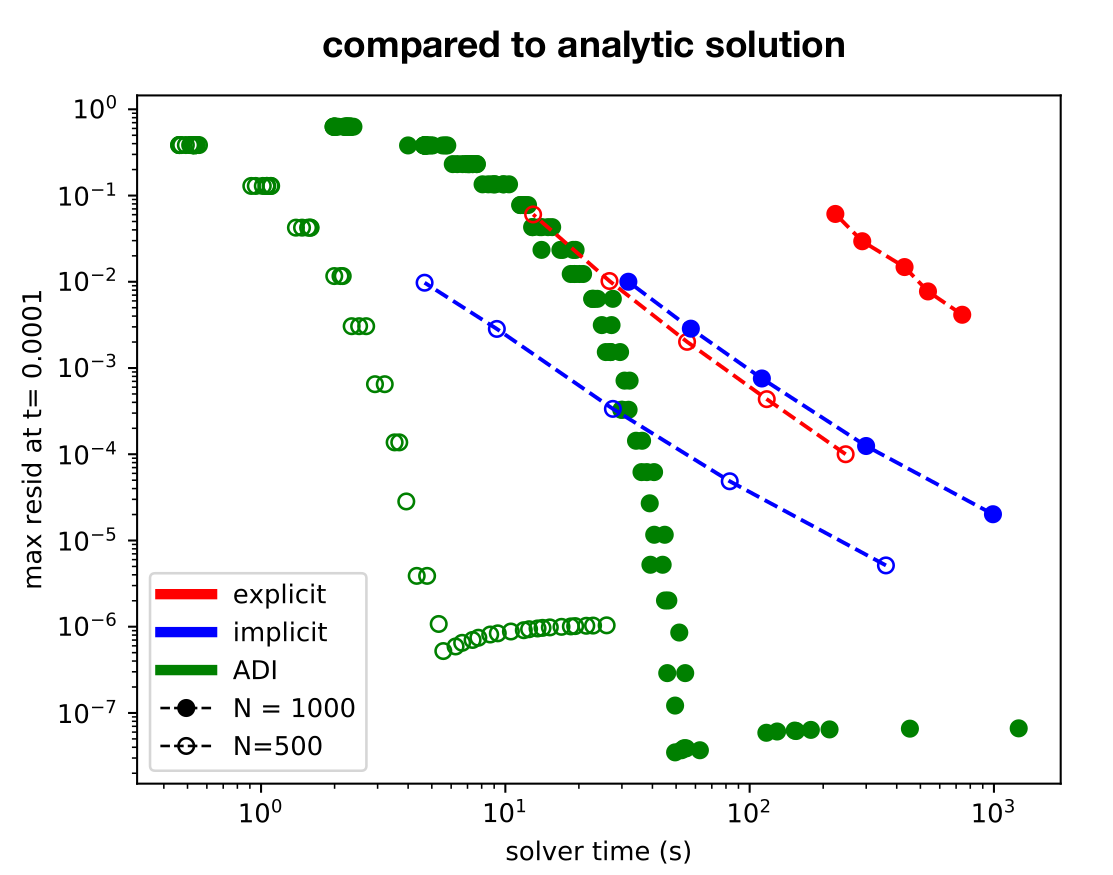
\includegraphics[width = 12cm]{time-err-plot.png}
	\caption{Execution time vs. errors of different methods}
\end{figure}
\end{document}

